\newcommand{\fig}[2]{\includegraphics[width=#1\textwidth]{#2}}
\newcommand{\centerfig}[2]{\begin{center}
\color{black} \includegraphics[width=#1\textwidth]{#2}\end{center}}
\newcommand \bnfdef  {\mathrel{::=}}
\newcommand \bnfalt  {\mathrel{|}}
\newcommand \tc[3]{{#1} \vdash {#2} : {#3}}

\section{Introduction}
Static and dynamic type systems for languages have their own distinct advantages. For instance, a static type system enables early error detection and enforces a certain extent of code style within a collaborative setting. On the other hand, the lightweight workflow associated with dynamic typing is highly suited for rapid prototyping and iterative approaches. Over the past several decades, researchers in the programming language community have been working on integrating aspects of both static typing and dynamic typing with the goal of allowing programmers access to advantages of both type systems. Gradual typing---originally proposed by \citet{siek2006gradual}---is one such solution that combines the two type systems and allows the end-users to optionally provide typing information. In recent times, it has largely gained traction in the programming language community and has been adopted by many programming languages both within industry and academia. Certain examples include Typed Racket \cite{tobin2006interlanguage}, TypeScript \cite{bierman2014understanding} and Reticulated Python \cite{vitousek2014design}.

\section{Advantages of Octave}
\subsection{Octave Is Relevant}
Octave is an open-source scientific programming language that uses a dynamic type system. It is widely employed in the domain of statistics, mathematics and machine learning for idea validation and fast prototyping. Octave shares the vast majority of its syntax and functionality with MATLAB, including but not limited to aspects such as having matrices as fundamental data type, built-in support for complex numbers, built-in math functions with extensive function libraries, and extensibility of user-defined functions \cite{wikibooks}. Therefore there is already a large audience and domain to potentially engage with for the proposed project. Note that in the context of domain research for the current discussion, we likewise refer to several supporting sources for MATLAB due to the near-analogous properties of the two languages.

\subsection{Octave Benefits From Gradual Typing}
In a paper describing program specializations used to produce efficient function overloading in Octave \cite{olmos2003turning}, Olmos et al. clearly illustrate the benefits of introducing static type-checking and shape analysis into Octave. In their work, static type and shape inferencing is used to directly reduce the number of type and shape checks needed at runtime and in doing so they can improve the efficiency of existing code. Functions and operators are highly overloaded in Octave to provide a simple interface for the end-users; however, the inevitable tradeoff for this flexibility is computational performance at runtime. The runtime system is responsible for type-checking, array shape determination, function call dispatching, and handling possible runtime errors. Hence Octave suffers from a number of computational inefficiencies that may be improved provided additional static type and shape context during the compilation step.

\section{Advantages of Gradual Typing}
In this section, we highlight several advantages of introducing a gradual type system to an existing dynamically-typed programming language such as Octave.

\subsection{Gradual Typing Incorporates Advantages from Static and Dynamic Typing}
It is widely acknowledged that static and dynamic type systems have their respective benefits and drawbacks. For instance, a static type system allows mistakes in a computer program to be caught at an earlier stage, preventing fatal errors in production environments. In contrast, bugs in a dynamically-typed language can usually only be detected at runtime, requiring numerous unit tests to ensure the correctness of a single piece of code. On the other hand, dynamically-typed languages are usually more flexible and accept various disciplines or coding practices, making them more suitable for tasks like idea validation, fast prototyping and scripting. Static typing, however, enforces certain coding disciplines and some degree of abstraction, which forces programmers to consider these design questions from the very beginning. Therefore, there are sure benefits and pitfalls that exist within both type systems.

In a gradual type system, programmers are able to decide which regions of code in a computer program are statically or dynamically typed, making different pieces suitable for different stages and scenarios \cite{siek2006gradual}. The Blame-Subtyping Theorem implies that statically-typed regions in a gradual type system cannot be blamed for type-casting errors and are therefore easy to analyze \cite{siek2015refined}. Hence, computer programs written in a gradually-typed languages take advantage of static typing in some regions while enjoying the flexibility of dynamic typing in other regions, integrating the benefits from both type paradigms in a single program simultaneously.

\subsection{Gradual Typing Enables Evolution of Programs}
Due to flexibility of dynamically-typed programming languages, it is common in industry that programs are initially developed in a dynamically-typed programming language for reasons like fast prototyping, idea validation and scripting. However, dynamically-typed programming languages usually expose programs to safety and security issues, which sometimes lead to fatal errors and even monetary losses in production environments. Furthermore, the runtime performance of dynamically-typed programs is unable to compete with that of statically-typed languages as static type systems are able to check many aspects of computer programs well before they execute. In order to resolve the issues mentioned above, prototyping programs in industry are sometimes refactored to statically-typed languages, in order to reduce the possibility of errors as well as to enhance runtime performance.

This process, nevertheless, is undoubtedly time-consuming and error-prone. The gradual guarantee ensures that computer programs remain well-typed as long as type annotations are correctly added \cite{siek2015refined}. The opposite---removing type annotations from a program does not break programs---is likewise always guaranteed in a gradual type system \cite{siek2015refined}. Therefore with the aid of gradual typing, programmers are able to gradually evolve their programs from untyped to fully-typed with type annotations without ever breaking the programs.

\section{Related Projects}
 
\subsection{Optimizing Function Overloading in Octave}
Octave and MATLAB were designed to be easy to use and have syntax that follow closely with mathematical notation. However, with dynamic type-checking, there are issues such as efficiency and the quality of the generated code. As briefly alluded to before, \citet{olmos2003turning} specifically address overloading in dynamically typed Octave programs. It introduces static typing for overloaded functions by making it explicit and restricting the input and output types of functions to match the actual function call. The main disadvantage to this approach is that the resulting Octave syntax is no longer as close to mathematical notation as before. However, by inferring the types used in the program for static typing, the system does not require any additional annotations from the user; hence the user developing their program is not greatly impacted. Since transformed program is statically typed, the overall computational performance of the system is improved. Thus, this paper shows how mixing dynamic and static typing can improve the overall system for Octave.

\subsection{Diamondback Ruby (DRuby)}
Diamondback Ruby \cite{furr2009combining} is an extension to Ruby with an optional static type system implemented by type inference. Programmers are able to annotate Ruby programs with type annotations, which will be checked by DRuby at runtime using contracts and blamed properly. It is also worth noting that DRuby is able to infer types on dynamic meta-language constructs, such as {\tt eval}, through a combined static and dynamic analysis \cite{druby}.

Although both DRuby and our proposed project aim to add an optional type system to an existing dynamically-typed language, there are some differences between the two projects. For instance, because DRuby uses static type inference to analyze Ruby programs, it requires static type-checking for the entire program. That is, some Ruby programs does not type-check in DRuby. This design, however, violates the criteria for gradual typing, which says gradual type systems must accept both fully untyped programs and fully typed programs \cite{siek2015refined}.  Our proposed gradual type system to Octave, in contrast, allows Octave programs to be partially type-checked; that is, some regions of Octave programs are able to remain dynamic.

That being said, we can still learn much from the DRuby project. In the future, type inference could also be added to our proposed type system to Octave \emph{together with gradual typing}. \citet{garcia2015principal} introduce a new approach to apply type inference on a gradually-typed language, admitting parametric polymorphism. In addition, the annotation syntax for DRuby is similar to informal documentation of Ruby, which facilitates programmers to annotate their Ruby programs. We will use this syntax as a reference when designing our annotation syntax for Octave.

\section{Project Distinction and Novel Aspects}
There are currently no gradual typing projects for Octave, and from the discussion above we have identified several advantages in applying gradual typing to the language.

By introducing optional syntactic forms for type specification, the goal is for users to gradually transition away from pure dynamically-typed codebases while also maintaining the flexibility to leave certain pieces untouched.

Additionally, previous projects such as \citet{chauhan2003type} and \citet{olmos2003turning} have largely abstracted the underlying program specializations away from the user and are largely ignored during development time until compilation. These do not intend to provide alternate workflows for the programmer but instead aim to offer methods to produce optimized code for execution. Thus, the intent here differs slightly from the projects mentioned. Rather than focusing primarily on the performance benefits that can be created through applying static reasoning over provided code, we hope to introduce a new type paradigm for the Octave programming language that is core to the user experience and provides an additional set of tools for the developers that enables them to directly add static type and shape guards. In this sense, our design deviates in that it encourages users to approach development differently and to use static types as much as possible, though we still ensure that existing code is able to run as is.

In fact, there are also performance benefits to adopting a gradual typing approach, in addition to the previous telescoping and program specialization techniques employed above. We again cite that recent development of gradually-typed compilers have been successful in attaining performance on par with statically-typed compilers \cite{kuhlenschmidt2018efficient}. As a result, the Octave variant that we propose will for additional optimizations in the compile phase and therefore have at least equal or better performance to existing compilers in general depending on the proportion of statically-typed code.

\section{Proof-of-Concept}
For the full proof-of-concept, see the project repository at \url{https://github.com/yuchong-pan/cpsc-311-project}. Below, we provide a tutorial for building the pipeline used to type-check our proposed gradually-typed Octave source files. To demonstrate the entire process of conversion from source code to a check result, we will show various stages of output as it is processed through our application. Figure \ref{fig:overview} illustrates an overview of the final structure of our proposed project.

\begin{figure}[h]
    \centering
    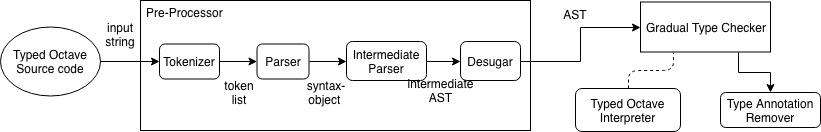
\includegraphics[width=.5\textwidth]{overview.jpg}
    \caption{Overview of Our Proposed Project}
    \label{fig:overview}
\end{figure}

\subsection{Pre-processing}
Before we begin static analysis of type information for a source file, we must convert it to our abstract representation. The four main stages of parsing include 1) tokenization 2) parsing to a Racket syntax object 3) parsing the object to an intermediate syntax 4) desugaring into our final abstract syntax tree. As the first two steps are largely coupled, we address them together in a single section below.

\subsubsection{Tokenization and Parsing}
For this proof of concept, we decided to perform our own lexical analysis and parsing using modified syntax that defines a subset of Octave with type information. However, we note that future work could be done to extend the official Octave open source parser \cite{johneaton2018octaveparser} to handle this stage for completeness. Figure \ref{fig:bnf} includes examples of rules used in our BNF.

\begin{figure}[h]
    \begin{lstlisting}
octave
        : translation_unit
        | octave translation_unit
        ;

translation_unit
        : statement_list
        | FUNCTION function_declare eostmt
          statement_list eostmt ENDFUNCTION
          eostmt
        ;

primary_expression
        : typed_identifier
        | BOOLEAN
        | CONSTANT
        | STRING_LITERAL
        | '(' expression ')'
        | '[' ']'
        | '[' array_list ']'
        ;
    \end{lstlisting}
    \caption[]{Selected BNF rules}
    \label{fig:bnf}
\end{figure}

We begin this stage by performing both lexical analysis and parsing using tools from the Racket brag library \cite{bragdocs}. In the first step of pre-processing, we load Octave source code into memory as a string and perform lexical analysis using a lexer function. For this, we have defined tokens for each of the terminals defined in the language such as for identifiers, constants, as well as literal characters.

The result of passing the source code string to this method is a generator function that, when called, generates a token list such as the one pictured in Figure \ref{fig:token}.

\begin{figure}[h]
    \begin{lstlisting}[language=racket]
(list
 (token-struct 'IDENTIFIER "a" #f #f #f #f #f)
 (token-struct 'WHITESPACE " " #f #f #f #f #t)
 (token-struct '= "=" #f #f #f #f #f)
 (token-struct 'WHITESPACE " " #f #f #f #f #t)
 (token-struct 'CONSTANT "3" #f #f #f #f #f))
    \end{lstlisting}
    \caption[]{Sample token list}
    \label{fig:token}
\end{figure}

Using the brag module, we obtain a parse function from the language file shown above which takes in a token list (or generator function) and ultimately constructs a syntax object \cite{racketstxobj} which provides an easily traversable form for us to desugar. The syntax in Figure \ref{fig:syntax} form is an abstract representation of the input source file in terms of the defined BNF. 

\begin{figure}[h]
    \begin{lstlisting}[language=racket]
'(octave
  (octave
   (translation_unit
    "function"
    (function_declare
     (func_return_list
      "["
      (func_ident_list
       (func_ident_list (typed_identifier "outx"))
       ","
       (typed_identifier "outy"))
      "]")
     "="
     ;; ...
    \end{lstlisting}
    \caption[]{Sample syntax structure}
    \label{fig:syntax}
\end{figure}

\subsubsection{Intermediate Representation}
Now that we have a structure that can be easily traversed by Racket, we are ready to transform the parsed syntax entity to an intermediate abstract syntax tree. Below we provide brief example structures that are used for this syntax, though we elaborate more on these in the main section to follow on type-checking.

To generate the abstract syntax tree, we use the PLAI Scheme language \cite{plaischeme} to match on the syntax structures produced by the previous step. To do this, we split each syntax object into a list using the syntax->list operation and this effectively allows us to parse 1) the current rule 2) the arguments for the rule.

We then extract the meaningful information captured within each rule, and produce a list of statement or function entities that describe the static form of the program. This includes any typing information that was declared within the source code. Figure \ref{fig:intermediate} is the example intermediate syntax obtained from this step.

\begin{figure}[h]
    \begin{lstlisting}[language=racket]
(list
 (i-func
  (i-id-type 'f 'dynamic)
  (list (i-id-type 'y 'dynamic)
        (i-id-type 'x 'dynamic))
  (list (i-id-type 'outy 'dynamic)
        (i-id-type 'outx 'dynamic))
  (list
   (i-assn-decl (list (i-id-type 'outx 'dynamic))
                      (i-id-type 'y 'dynamic))
   (i-assn-decl (list (i-id-type 'outy 'dynamic))
                      (i-id-type 'x 'dynamic))))
 (i-assn-decl
  (list (i-id-type 'x 'dynamic))
  (i-app (i-id-type 'f 'dynamic)
         (list (int 1) (int 2)))))
    \end{lstlisting}
    \caption[]{Intermediate syntax for source code}
    \label{fig:intermediate}
\end{figure}

\subsubsection{Desugaring}
Finally, we must desugar the intermediate syntax into the final abstract syntax. In this stage, one major goal is to insert declarations for variable assignments as they are being assigned to. We do this by scoping variables to environments and performing lookups to find ``unbound'' variables that are being assigned to. Once bound, the type of the variable is fixed from that point onwards. Additionally, in the process of converting to the abstract syntax we strip off unnecessary type information that can be bundled with identifiers.

At this point, the original source file has been transformed into our desired form and we can perform type-checking on it. In the section to follow, we will elaborate on the form and use of our abstract syntax.

\subsection{Type-Checking}

\subsubsection{Type Consistency}
\label{sec:consistency}
One can view dynamic typing as a type system with only one type {\tt dynamic}. Thus, the main difference of a gradual type system from a static type system is the additional unknown type, denoted by {\tt ?}, which is used to indicate a partially-known structure of a type \cite{siek2006gradual}. For instance, {\tt int $\to$ ?} represents a function type whose domain is {\tt int} and whose co-domain can be any type.

In order to support the unknown type, the type equality relation is no longer working in a gradual type system. Consider a function {\tt f} with type {\tt int $\to$ int}, and a variable {\tt x} with type {\tt ?}. A gradual type system should allow {\tt f} to be applied on {\tt x} by casting $x$ from type {\tt ?} to type {\tt int} in the runtime, whereas type {\tt ?} is not equal to type {\tt int}. Hence, an important difference of a gradual type system froma static type system is to replace the type equality relation with the type consistency relation \cite{siek2006gradual}, which is defined in Figure {fig:consistency}. Here, the arrow type {\tt ($\rightarrow$ T T)} is an explicit function type, and the star type {\tt T $\times$ T} is the type for pairs of two instances of difference types.

\begin{figure}[h]
    \[\begin{array}{rcl}
        B & \bnfdef & \texttt{int} \bnfalt \texttt{bool} \bnfalt \texttt{string} \\
        T & \bnfdef & B \bnfalt \texttt{($\rightarrow$ T T)} \bnfalt \texttt{T $\times$ T} \bnfalt \texttt{?} \bnfalt \texttt{none}
    \end{array}\]
    \caption{Type definitions}
    \label{fig:types}
\end{figure}

\begin{figure}[h]
    \begin{mathpar}
        \infer{~}{\texttt{?} \sim T}
        \qquad \infer{~}{T \sim \texttt{?}}
        \qquad \infer{~}{B \sim B} \\
        \qquad \infer{T_1 \sim T_3 \quad T_2 \sim T_4}{T_1 \to T_2 \sim T_3 \to T_4}
        \qquad \infer{T_1 \sim T_3 \quad T_2 \sim T_4}{T_1 \times T_2 \sim T_3 \times T_4}
    \end{mathpar}
    \caption{Type consistency rules}
    \label{fig:consistency}
\end{figure}

The type consistency relation needs to respect several properties. First, type consistency should \emph{conservatively} extend the type equality relation \cite{garcia2016abstracting}. Described as a criterion for gradual typing, a gradual type system should behave exactly the same as a static type system for fully statically-typed programs \cite{siek2015refined}. Hence, two basic types $T_1$ and $T_2$ are consistent if and only if they are equal. Second, it is easy to see that type consistency should be reflexive, symmetric, but not transitive. To see the non-transitivity, if consistency were transitive, then {\tt int $\sim$ ?} and {\tt ? $\sim$ bool} would imply that {\tt int $\sim$ bool}, which would violate the criterion for gradual typing stated above. In our type-checker, we implemented the helper function {\tt consistent?} to check type consistency of two types, given in Figure \ref{fig:consistent}.

\begin{figure}[h]
    \begin{lstlisting}[language=racket]
(define (consistent? T1 T2)
  (match `(,T1 ,T2)
    [`(,T1 dynamic) #t]
    [`(dynamic ,T2) #t]
    [`(,(arrow T1-dom T1-cod)
       ,(arrow T2-dom T2-cod))
     (and (consistent-list? T1-dom T2-dom)
          (consistent-list? T1-cod T2-cod))]
    [else (equal? T1 T2)]))
    \end{lstlisting}
    \caption[]{Helper function to check type consistency}
    \label{fig:consistent}
\end{figure}

\subsubsection{Typing Rules}
Figure \ref{fig:types} is the typing rules that we follow in the proof-of-concept stage. It extends the type system of the gradually-typed lambda calculus (GTLC) \cite{siek2006gradual}. The typing rules described in Figure \ref{fig:types} can be read as ``if the propositions above the bar are true, then the proposition below the bar will be true'', and the type judgements ``$\tc{\Gamma}{e}{T}$'' can be read as ``expression $e$ has type $T$ in the context $\Gamma$''. The metafunction $fun$ extracts the domain and co-domain from a possible function type (i.e., the {\tt ?} type can be viewed as a function type {\tt ? $\to$ ?}).

The main extension of our type system to the GTLC type system is the addition of statements because Octave is an imperative language. Statements include assignments and if-statements and do not have types. We represent typing rules for assignments and for if-statements in Figure \ref{fig:stmt-typing}. An assignment type-checks if the type of the left-hand side variable and the type of the right-hand side expression are consistent. An if-statement type-checks if the condition expression has the {\tt bool} type.

\begin{figure}[h]
    \begin{mathpar}
        \infer{\tc{\Gamma}{e_1}{T_1} \quad \tc{\Gamma}{e_2}{T_2} \\ fun(T_1) = T_{11} \rightarrow T_{12} \quad T_2 \sim T_{11}}{\tc{\Gamma}{\texttt{$e_1$($e_2$)}}{T_{12}}} \\
        \infer{\tc{\Gamma}{e_1}{\texttt{int}} \quad \tc{\Gamma}{e_2}{\texttt{int}}}{\tc{\Gamma}{\texttt{$e_1$ + $e_2$}}{\texttt{int}}} \\
        \ldots \\
        \begin{array}{rcl}
            fun(T_1 \to T_2) &=& T_1 \to T_2 \\
            fun(\texttt{?}) &=& \texttt{?} \to \texttt{?}
        \end{array}
    \end{mathpar}
    \caption{Expression typing rules}
    \label{fig:expr-typing}
\end{figure}

\begin{figure}[h]
    \begin{mathpar}
        \infer{\tc{\Gamma}{x}{T_1} \quad \tc{\Gamma}{e}{T_2} \quad T_1 \sim T_2}{\texttt{$x$ := $e$}} \\
        \infer{\tc{\Gamma}{e}{\texttt{bool}}}{\texttt{if $e$ then $s_1$ else $s_2$ endif}} \\
    \end{mathpar}
    \caption{Statement typing rules}
    \label{fig:stmt-typing}
\end{figure}

\subsubsection{Abstract Syntax Tree (AST)}
In our abstract syntax tree (AST), statements will be defined as all of the statements we want to support in type-checking, such as expressions, declarations, assignments, function definitions, and if-statements. Note that expressions are always associated with types, whereas statements that are not expressions do not have types.

An important AST node is the function definitions. Unlike many other programming languages, Octave requires us to specify both the identifiers for arguments and those for return variables. Therefore, in our proposed gradual typing extension to Octave, that means both the input and output parameters can be type annotated. To represent that, we use a pair of a symbol and a {\tt Type} type to represent each argument and each return variable and store them in two lists. The body of the function may also need to be type-checked. We can achieve that by creating a list of statements to represent the body. This way, we can recursively call the type-checker for statement to type-check the body of a function.

\begin{figure}[h]
    \begin{lstlisting}[language=racket]
(struct func
  ([name : Symbol]
   [args : (Listof (Pair Symbol Type))]
   [rets : (Listof (Pair Symbol Type))]
   [body : (Listof Stmt)]))
    \end{lstlisting}
    \caption[]{AST node for {\tt func}}
    \label{fig:func}
\end{figure}

Now that we have an idea of how to represent Octave programs as an AST, we can use pass this AST into our type-checker to check for type consistency. 

\subsubsection{Type-Checker Implementation Details}
{\bf Type Environments.} When a variable or a function is declared, we allow users to specify the type of the variable or the function. However, we need to be able to retrieve this information when we type-check statements and expressions. In order to keep track of what the types of the variables are, we introduce an environment that stores this data. An environment can be represented as {\tt (define-type Env (Listof (Pair Symbol Type)))}. Everytime we encounter a declaration or a function definition, we can append a pair of an identifier and its corresponding type to the environment. Now, we can thread the environment through our program so it can be accessed by statements and expressions. When we get to type-checking a statement or an expression, we can look up the variable name in the environment to retrieve its type. With this environment passed around, we can complete the type-checker. 

{\bf Statements and Expressions.} Our type-checker is broken down into two helper functions to type-check statements and expressions, respectively. Note that the type of an expression will be used to type-check the super-expression that contains it. For instance, to typecheck the expression {\tt $e1$ + $e2$}, we need to ensure that $e1$ and $e2$ both have type {\tt int}. Therefore, the type-checker needs to type-check each sub-expression and returns the type information of the expression.

In contrast, non-expression statements cannot be further operated on and therefore do not have types. However, it is worth noting that two types of statements, namely declarations and function definitions, will update the type environment; i.e., they will bind new identifiers to their corresponding types in the environment. Therefore, the type-checker for statements returns the possibly updated type environment.

{\bf Case Study: Assignments.} We will look at one of the more interesting cases such as type-checking an assignment, because Octave allows multiple variables at the left-hand side of an assignment. The type-checker implementation for assignments is given in Figure \ref{fig:assn}. With an assignment, we first need to determine the types of the left-hand side variables. To do that, we create a list of expected types by searching in the environment and throwing an error if any of the variables are not found. If an error occurs, that would mean this assignment was invalid since we have never declared this variable before. Then, we need to get the actual types. Since the right-hand side of an assignment is an expression, we can call our helper function {\tt typecheck-expr} to type-check the right-hand side.

Note that Octave allows the left-hand side of an assignment to have less variables than the number of values on the right side of the assignment, in which case Octave ignores the last several output values that are missing on the left-hand side. We model this in our type-checker by comparing the length of both sides of the assignment and removing the unnecessary output types from the function application if the length on the right is greater than the length on the left. After this, we also need to make sure the left-hand side of the assignment does not have more variables than the right side of the assignment. For example, we can't have {\tt x, y = 1}. In this case, we will throw an error. If all of the length checks pass, we can simply call our consistent function on the list of types which will check for type consistency between the left-hand side and the right-hand side of the assignment.  

\begin{figure}[h]
    \begin{lstlisting}[language=racket]
[(assn names expr)
 (local
    [(define expect-types
       ((inst map Type Symbol)
        (lambda (name)
          (local [(define result (assoc name env))]
            (if (false? result)
                (error 'typecheck-stmt "...")
                (cdr result))))
        names))
     (define expect-length (length expect-types))
     (define actual-types
       (local
         [(define original
            (typecheck-expr env expr))
          (define listify
            (if (list? original)
                original
                (list original)))]
         (if (> (length listify) expect-length)
             (take listify expect-length)
             listify)))
     (define actual-length (length actual-types))]
   (cond
     [(not (= expect-length actual-length))
      (error 'typecheck-stmt "...")]
     [(consistent-list? expect-types actual-types)
      env]
     [else
      (error 'typecheck-stmt "...")]))]
    \end{lstlisting}
    \caption[]{Type-checking case for assignments}
    \label{fig:assn}
\end{figure}


{\bf Case Study: Function Applications.} Function applications are another interesting case that is worth studying. The type-checker implementation for assignments is given in Figure \ref{fig:app}. Unlike some other languages, Octave allows the number of actual arguments of a functional to be different from the number of arguments declared in the argument list, and it allows functions to return multiple return values. Handling arguments of function applications is similar to handling assignments, as described above. Therefore, we need to truncate the actual argument list if necessary, and append dummy dynamic types to type-check missing arguments. Then, we check the type consistency between the actual argument list and the expected argument list using the type consistency rule for star types.

It is also worth noting that we may apply a function with the {\tt ?} type because the {\tt ?} type can also represent a function type. This may happen when we apply a higher-order function passed in as an argument of another function, where the type annotation of the argument is {\tt dynamic}. To type-check this case, we need to extract the domain type and the co-domain type of the {\tt dynamic} type, which are both {\tt dynamic} according to the metafunction $fun$ is the type consistency rules in Figure \ref{fig:consistency}. Therefore, we implemented two helper functions, {\tt fun-dom} and {\tt fun-cod} to extract the domain and the co-domain of a possible function type.

\begin{figure}[h]
    \begin{lstlisting}[language=racket]
[(app fun args)
 (local [(define fun-type (typecheck-expr env fun))]
   (if (or (arrow? fun-type)
           (equal? fun-type 'dynamic))
       (local
         [(define expect-types
            (fun-dom fun-type))
          (define actual-types
            (typecheck-list env args))
          (define expect-length
            (length expect-types))
          (define actual-length
            (length actual-types))
          (define adjusted-actual
            (cond
              [(> actual-length expect-length)
               (take actual-types expect-length)]
              [(< actual-length expect-length)
               (append
                actual-types
                (build-list (- expect-length
                               actual-length)
                            (lambda (x)
                              'dynamic)))]
              [else actual-types]))
           (define return-types
           (fun-cod fun-type))]
         (if (consistent-list? expect-types
                               adjusted-actual)
             return-types
             (error 'typecheck-expr "...")))
       (error 'typecheck-expr "...")))]))

(: fun-dom (-> Type (Listof Type)))
(define (fun-dom fun-type)
  (cond
    [(arrow? fun-type) (arrow-dom fun-type)]
    [(equal? fun-type 'dynamic) '(dynamic)]
    [else (error 'fun-dom "...")]))

(: fun-cod (-> Type (Listof Type)))
(define (fun-cod fun-type)
  (cond
    [(arrow? fun-type) (arrow-cod fun-type)]
    [(equal? fun-type 'dynamic) '(dynamic)]
    [else (error 'fun-cod "...")]))
    \end{lstlisting}
    \caption[]{Type-checking case for function applications}
    \label{fig:app}
\end{figure}

The rest of the type-checking cases are very similar and simpler than the two cases we described above. They can be implemented by calling the helper functions for statements and expressions as well as calling the consistency function to check the consistency of two types.

\section{Plan for Next Steps}
As the next step to meet the team's full project goals, and in a fashion akin to both TypeScript and typing aspects, we will compile the augmented Octave scripts back to the original syntax to be run. In order to compile the typed Octave code into executable Octave code, we will recursively generate Octave code directly from our high-level AST. We believe that this will be a manageable task as, given instances of our AST representation, there is sufficient information to re-create the original semantics. This is beneficial because not only can a user type check their code, they can also execute the type checked code in their original environment. However, we approach this with the hope that in the future a compiler that capitalizes on the performance benefits may be developed as a follow-up project; though this is out of scope for the current project.

In addition, we intend to enrich and further introduce nuances into our gradual typing scheme by delving into features such as static dimension checking provided that matrices are a core component of the language domain. Octave can include matrices to do mathematical calculations such as element operations, vector operations, and other ways to manipulate matrices. We believe that this is a challenging task given that we introduce the notion of shapes as an additional constraint to our type checking. Furthermore, there will inherently be many syntactic ambiguities introduced to parsing. One such example is the ambiguity between matrix extraction and regular function call, another is simply the matter that many primitive operators such as arithmetic operators are heavily overloaded in Octave and so correctly capturing the surrounding context is an important matter.

For this task, we now propose the following preliminary syntax for matrices and lists (which we treat as a simple desugaring to a 1 by n matrix):
\begin{align*}
& \text{\tt identifierA : matrix[Type][n, m]} \\
& \text{\tt identifierB : list[Type]}
\end{align*}

For example, if we had {\tt m:matrix[int][2,2] = [1,2; 3,4]}, this will successfully type check. In contrast, if we have  {\tt m:matrix[int][2,2] = [1,2; 3,4; 5,6]}, this will violate the dimension check as we create a 3x2 matrix instead of the declared 2x2. Additionally, {\tt m:matrix[string][2,2] = [1,2; 3,4]} will violate the type consistency of the matrix. Since we are introducing gradual typing, we will also allow {\tt matrix[2,2] = [1,2; 3,4]} which would allow any type to be assigned to the matrix.

We hope to create a meaningful and useful tool for Octave developers to use and ideally contribute towards in the future.

\section{Concluding Remarks}
Octave is an ideal candidate language as it is a well-known and relevant language, it benefits from the process of gradual typing and has many reference resources. In this proof of concept we provided an overview of the the stages of work we've implemented for the pre-processing as well as type-checking stages. For each stage, we elaborate on the respective tools used and steps taken to achieve certain inputs and outputs. We've also included snippets of the source code to reinforce users' understanding of how to recreate the proof-of-concept without serious difficulties in a tutorial-like format.

The objective for this project is to develop a gradually-typed variant for Octave that sufficiently expresses the basic data types of the language. We believe that the flexible nature of gradual typing offers great value to data scientists and various users of Octave in that it remains an effective prototyping tool while optionally providing compile-time type and invariant assertions. To achieve this, we intend to base our initial prototypes for static semantics on the existing literature described above.

\appendix

\begin{acks}
    The authors would like to thank the course staff of CPSC 311 at University
    of British Columbia for their feedback.
\end{acks}
